\chapter{Grundlagen}

\printmyminitoc{1}

\section{CAN-Bus}
Bei einem Can-Bus handelt es sich um eine serielle Netzwerktechnologie, 
welche mehrere Geräte mit einem Draht verbindet.
Die Entwicklung des Can-Bus wurde von Bosch im Jahr 1983 begonnen. 1986 wurde der erste Can-Bus Standard 
veröffentlicht.
Die Motivation der Entwicklung war die effiziente Kommunikation zwischen den Steuergeräten in einem Auto. 
Als günstige
Nebenwirkung konnte damit die Kabelmenge reduziert werden, da alle Geräte mit einem Bus verbunden werden können.
Durch die höhere Zuverlässigkeit und Funktionalität des Can-Bus, wurde dieser schnell in der Autoindustrie etabliert.
Aber auch in anderen Sektoren, wie z.B. der Medizintechnik, der Gebäudeautomation oder der Luftfahrt, spielt der
Can-Bus mittlwerweile eine wichtige Rolle.
\cite[Seiten 2-10]{Voss2008}
\\
Man sprich von einem Bussystem, da alle Geräte gleichberechtigt sind. Dass heißt, dass jedes Gerät Nachrichten 
senden und empfangen kann.
Die Nachrichten werden nach Broadcasting-Prinzip übertragen. Jede Nachricht wird von allen Knoten empfangen, 
aber nur die Knoten, die die Nachricht benötigen, verarbeiten sie. Diese werden nicht Einhaltung der Protokollregeln 
überprüft,
da dies zu einer größeren unnötigen Last auf dem Bus führen würde. 
Jedoch wird die Integrität der Nachrichten durch eine Prüfsumme sichergestellt. Das wird auch mit 
einer Acknowledge-Nachricht(ACK) bestätigt. Wird eine Nachricht nicht bestätigt, wird von dem Sender eine Fehlermeldung
auf den Bus gesendet.
Bei einer fehlerhaften Nachricht reagieren
die Knoten mit einer Fehlermeldung, die wieder der gesamte Bus empfängt. Wenn ein Knoten dauerhaft fehlerhafte
Nachrichten sendet, wird dieser vom Bus getrennt. Die auf dem Bus gesendeten Daten werden mit einer Nachrichten-ID
versehen, die die Priorität der Nachricht angibt. Die Nachrichten mit der niedrigsten ID haben die höchste Priorität.
Die Maximale Länge einer Nachricht beträgt 8 Byte. Durch die vergleichsweise geringe Länge der Nachrichten, kann 
eine geringe Latenz erreicht werden. Dabei kann eine höchste Baudrate von 1Mbit/s gesetzt werden.
\cite[Seiten 13-19]{Voss2008}
\\
Alle Knoten in einem Can-Bus sind mit einem Zweiadrigen Kabel verbunden. Diese werden als High(CAN\_H) und Low(CAN\_L) 
bezeichnet. Der Bus ist an beiden Enden mit einem Widerstand von 120 Ohm abgeschlossen um Reflexionen zu vermeiden.
\cite[Seite 132]{Voss2008}
\\
Eine Nachricht auf einem CAN-Bus ist im allgemeinen in einem Can-Frame verpackt. Dieser beginnt
mit einem Startbit, welches Start of Frame (SOF) genannt wird. Darauf folgt das Arbitration Field, 
in dem die Nachrichten-ID und ein Bit RTR (Remote Transmission Request) gesetzt wird. Das RTR-Bit wird gesetzt,
wenn der Sender eine Antwort auf die Nachricht erwartet. Das Control Field wird für die Datengröße und die Nachrichtenlänge
verwendet. Im Data Field sind die eigentlichen Nutzdaten kodiert. Das CRC Field enthält eine Prüfsumme, welches die Richtigkeit
der Nachricht überprüft. Hier folgt ein ACK Field, welches die Prüfsumme bestätigt. Die Nachricht endet mit einem End of Frame (EOF).
Danacht folgt ein Interframe Space (IFS) von 3 Bit, welches eine Pause zwischen den Nachrichten darstellt.
\cite[Seite 36]{Voss2008}

\subsection{Erweitertes Can-Protokoll}
Das Standard Can-Protokoll hat einen 11 Bit Identifier, während das erweiterte Can-Protokoll 29 Bit Identifier
besitzt.
Die Society of Automotive Engineers (SAE) hat das J1939-Protokoll entwickelt, um die Kommunikation in Nutzfahrzeugen
zu verbessern. Der Fokus liegt auf der Kommunikation mit dem Antrieb des Fahrzeugs. Dafür wird der 11 Bit
Identifier mit J1939 auf 29 Bit erweitert um mehr verschiedene Nachrichten zu ermöglichen.\\
Auf einem Can-Bus können der Standard 11 Bit Identifier und der erweiterte 29 Bit Identifier gleichzeitig verwendet werden.
Wenn zwei Nachrichten den gleichen 11 Bit Identifier haben, wird die Nachricht mit dem 11 Bit Identifier bevorzugt immer die
höhere Priorität haben. Die spezifierten Baudraten sind hier 250kbit/s und 500kbit/s. Die Hauptkomponenten des
erweiterten Identifier sind die Priorität, eine Parameter Group Number (PGN) und eine Quell-Adresse.
Das PGN-Feld ist aus 1 Bit Data Page (DP), 1 Bit Extended Data Page (DP), einer Protocol Data Unit (PDU) und einem PDU spezifischen 
Feld (PS) aufgebaut. Die DP und EDP bestimmen mit welchem Standard die 
Nachricht gesendet wird. Für SAE J1939 werden aber nur zwei Kombinationen verwendet. 
Das PS-Feld kann entweder eine Zieladresse oder eine Gruppenerweiterung (GE) sein. Welches PS-Feld
verwendet wird, hängt von der PDU ab. Wenn diese einen Wert von unter 240 hat, wird das PS-Feld als Zieladresse verwendet. 
In dem anderen Fall wird das PS-Feld als Gruppenerweiterung verwendet.
\cite{Murvay2018}
\begin{figure}[H]
    \centering
    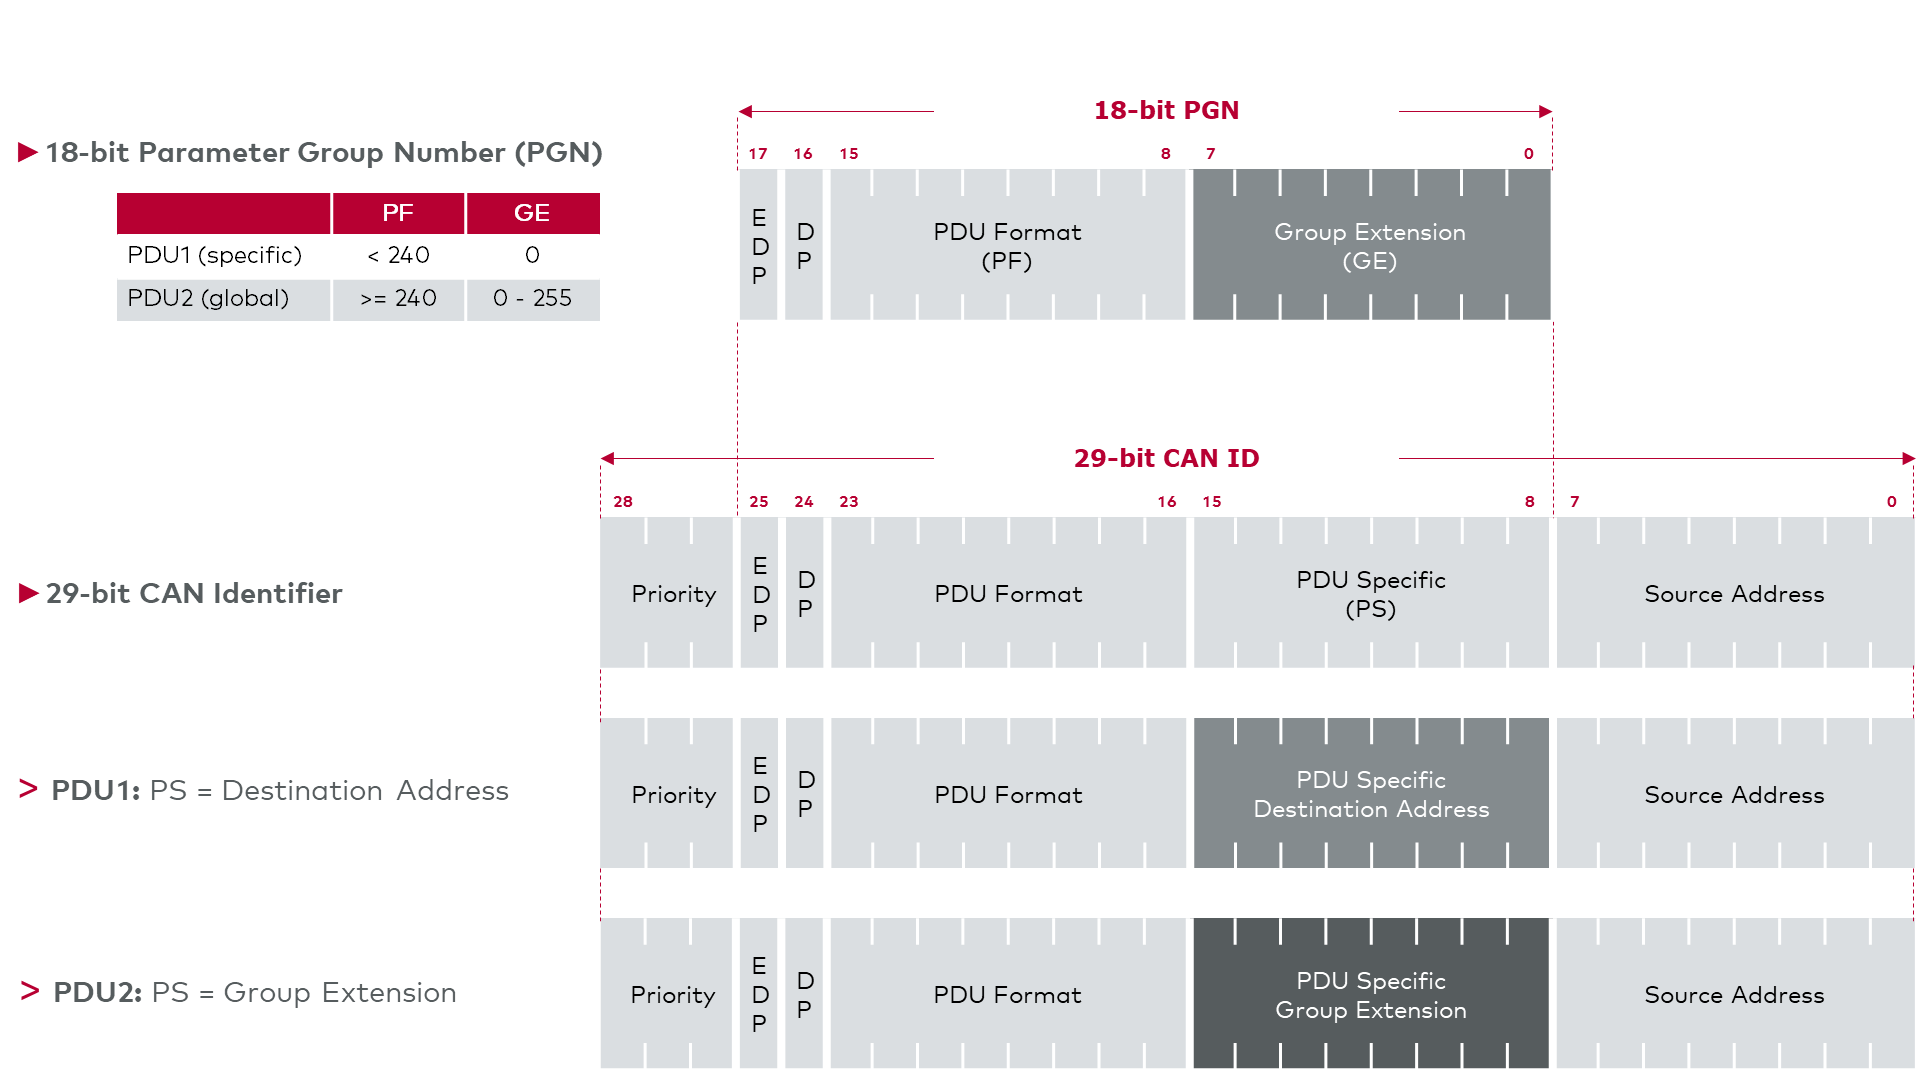
\includegraphics[scale=0.28]{images/j1939header.png}
    \caption{Header einer J1939-Nachricht auf dem CAN-Bus \cite{VektorSAE}(letzter Zugriff: 28.01.2025)}
    \label{fig:j1939header}
\end{figure}

Auch wenn in einem CAN-Bus jedes Gerät immer jede Nachricht empfängt, soll es durch die Zieladresse möglich sein,
dass nur das Gerät die Nachricht verarbeitet, welches die Nachricht benötigt. Um eine Nachricht an alle Knoten 
zu senden, wird die Zieladresse auf 255 gesetzt. Mit der Gruppenerweiterung ist es nicht möglich eine Nachricht 
zielgerichtet an bestimmte Geräte zu senden. \cite{Murvay2018}




\section{Raspberry Pi}
Ein Raspberry Pi ist ein Einplatinencomputer, der von der Raspberry Pi Foundation entwickelt wurde. 
Dieser den Prozessor mit Grafikeinheit, Arbeitsspeicher, Speicher und Anschlüsse auf einem einzigen Board integriert.
Es handelt sich um einen vollwertiger Computer, der kleiner als normale PCs ist. Für die Größe ist der Raspberry Pi
leitsungsstark, während er einen recht günstigen Preis von unter 100€ hat. Er kann mit einem normalen Betriebssystem
betrieben werden. Trotzdem gibt es ein spezielles Betriebssystem, das für den Raspberry Pi entwickelt wurde, das Raspberry Pi OS (ehemals Raspbian).
Dieses basiert auf der Linux-Distribution Debian. Um viele Funktionen erfüllen zu können, hat der Raspberry Pi viele Anschlüsse.
Der Raspberry Pi 5 hat 4 USB-Anschlüsse, 2 Micro-HDMI-Anschlüsse, 1 Ethernet-Anschluss, 1 USB-C-Anschluss für die Stromversorgung und einen Micro-SD-Kartensteckplatz.

\subsection{Raspberry Pi als Rogue Device}
Unter einem Rogue Device versteht man ein Gerät, welches sich unautorisiert und unauffällig in ein Netzwerk integriert. \cite{Scarfone2008}
Dies kann ein Raspberry Pi sein, der sich in ein Netzwerk einbindet und Daten abfängt oder manipuliert. Hierüber können 
sich Angreifer Zugriff auf das Netzwerk verschaffen. 
Ein solches Gerät kann dazu verwendet werden, um eigenen Code auszuführen, der beispielsweise Daten verändert oder 
weitere Angriffe vorbereitet. Zudem kann es von Angreifern aus der Ferne gesteuert werden, wodurch gezielte 
Manipulationen oder Spionageangriffe möglich sind. Darüber hinaus lässt sich ein Rogue Device nutzen, um Informationen 
über das Netzwerk zu sammeln, etwa durch das Mithören von Kommunikation oder die Analyse von Sicherheitsmechanismen.
Das ermöglicht es, Schwachstellen im Netzwerk aufzudecken und gezielt auszunutzen.

\section{State of the Art}
\begin{itemize}
    \item canCommander
    \item cantools: eine Python-Bibliothek, die es ermöglicht Can-Bus Nachrichten zu dekodieren
\end{itemize}
\subsection{Anbindung von Raspberry Pi an CanBus}
\begin{itemize}
    \item Raspbian OS hat seit 05.05.2015 eingebundenen Support für den Mikrochip MCP251x
\end{itemize}
\cite{Salunkhe2016}
\begin{itemize}
    \item PiCan2 ist ein CanBus Board für den Raspberry Pi
    \item HAT (Hardware Attached on Top) Standard
    \item erlaubt dem Raspberry Pi mit dem CanBus zu kommunizieren mit einer Geschwindigkeit von bis zu 1Mbit/s
    \item UCAN ist ein USB-CAN Adapter, der es ermöglicht ein beliebiges USB-Gerät mit dem CanBus zu verbinden
\end{itemize}
\cite{Pant2019}
\subsection{Übersetzung von CanBus Nachrichten}
\begin{itemize}
    \item J1939 (DBC-Dateien) (https://docs.fileformat.com/de/database/dbc/)
    \item NMEA 0183 
    \item NMEA 2000 $\rightarrow$ CanBoat (https://github.com/canboat/canboat)
    \item cantools Python Library 
    \item dbc Datei verstehen \href{https://www.csselectronics.com/pages/can-dbc-file-database-intro}{csselectronics}
\end{itemize}